

\documentclass[12pt,a4paper]{article}
\newcommand\persiangloss[2]{#1\dotfill\lr{#2}\\}
\usepackage{graphicx}
\usepackage{xcolor}
\usepackage{listings}
\usepackage{indentfirst}
\usepackage{float}
\usepackage[pagebackref=false,colorlinks,linkcolor=blue,citecolor=magenta]{hyperref}
\usepackage{xepersian}
\settextfont{XB Niloofar}
\definecolor{vgreen}{RGB}{104,180,104}
\definecolor{vblue}{RGB}{49,49,255}
\definecolor{vorange}{RGB}{255,143,102}

\lstdefinestyle{verilog-style}
{
	language=C,
	basicstyle=\small\ttfamily,
	keywordstyle=\color{vblue},
	identifierstyle=\color{black},
	commentstyle=\color{vgreen},
	numbers=left,
	numberstyle=\tiny\color{black},
	numbersep=10pt,
	tabsize=8,
	moredelim=*[s][\colorIndex]{[}{]},
	literate=*{:}{:}1
} 



\begin{document}
	\thispagestyle{empty}
	\vspace*{0mm}
	\centerline{
\includegraphics[height=4cm]{logo.png}}
	\vspace*{5mm}
	\begin{center}
		{\Huge
لوستر هوشمند - گزارش چهارم
}
\\[1cm]
آزمایشگاه سخت‌افزار
\\[1cm]
دانشکده مهندسی کامپیوتر
\\[4cm]
{\large
محمدرضا عبدی ۹۷۱۱۰۲۸۵

حمیدرضا کامکاری ۹۷۱۱۰۱۷۷

یگانه قره‌داغی 97106216
}
	\\[5cm]
	اردیبهشت ۱۴۰۱
	\end{center}
\newpage

\section*{گزارش چهارم}
هدف از این آزمایش این هفته، درست کردن رابط گرافیکی برنامه تنظیم لوستر بود. انواع تنظیمات ممکن لوستر برای کاربر در زیر آورده شده‌است:

\begin{itemize}
	\item 
{تنظیم حساسیت سنسور نوری:} کاربر می‌تواند با انتخاب عددی میان ۱۰ الی ۱۵۰ (توسط \lr{slidebar})، میزان حساسیت سنسور نور را تنظیم کند (عدد کمتر معادل حساسیت کمتر است؛ یعنی میزان نور با تغییرات بیشتری نسبت به عددی بیشتر تغییر می‌کند).
	\item 
{دکمه روشن و خاموش:} کاربر می‌تواند تمامی چراغ‌های لوستر (شاخه مورد نظر) را خاموش یا روشن کند.
	\item 
{حالت استاتیک یا داینامیک (\lr{Adaptive}):} کاربر می‌تواند با حالت استاتیک یک مقدار خاص را برای روشنایی انتخاب کرده و تمامی \lr{LED} های لوستر با آن مقدار تنظیم می‌شوند. در حالت داینامیک نیز مقدار روشنایی لوستر با سنسورهای تنظیم می‌شود.
	\item 
{تنظیم حداکثر و حداقل میزان روشنایی:} کاربر می‌تواند با انتخاب عددی میان ۰ تا ۲۵۵(توسط \lr{slidebar})، حداقل و حداکثر میزان روشنایی یک شاخه را تعیین کند. بنابراین روشنایی یک شاخه، محدود به این دو عدد می‌شود و نمی‌تواند مقداری خارج از این بازه بگیرد.
	\item 
{مودهای مختلف لوستر:} مودهای متفاوت که می‌توانند شامل لوستر را در حالت تنظیم داینامیک عادی یا رقص نور (همانند گزارش اول) تنظیم کنند (این حالت‌ها در قسمت‌های بعدی تکمیل می‌شوند). یکی از مودهای در نظر گرفته شده برای این قسمت حالت \lr{Inverted min to max} است که در آن نور دو شاخه به صورت معکوس با همدیگر کم و زیاد می‌شود.

\end{itemize}
همچنین برای ارتباط میان موبایل اپ و آردوییو به کمک ماژول \lr{ESP8266-07}، مدار را در مراحل زیر می‌بندیم (دقت کنید که هنگام آپلود کردن کد باید پین‌های \lr{RX} و \lr{TX} قطع شوند):
\begin{enumerate}
	\item
	پین \lr{RX} در ماژول \lr{ESP} را به پین \lr{TX} آردویینو متصل می‌کنیم.
	\item
	پین \lr{TX} در ماژول \lr{ESP} را به پین \lr{RX} آردویینو متصل می‌کنیم.
	\item
	پین \lr{CH\_PD} یا \lr{Enable} در ماژول \lr{ESP} را به پین \lr{+3V} آردویینو متصل می‌کنیم.
	\item
	پین \lr{VCC} در ماژول \lr{ESP} را به پین \lr{+3V} آردویینو متصل می‌کنیم.
\end{enumerate}

در نهایت می‌توان با نصب کردن برنامه موبایل و اتصال آن به \lr{ESP} و آردویینو، تنظیمات موردنظر را انجام داد.
\newpage
در شکل زیر می‌توان شماتیک اپلیکیشن موبایل را دید.

 \begin{figure}[H]
 	\centering
 	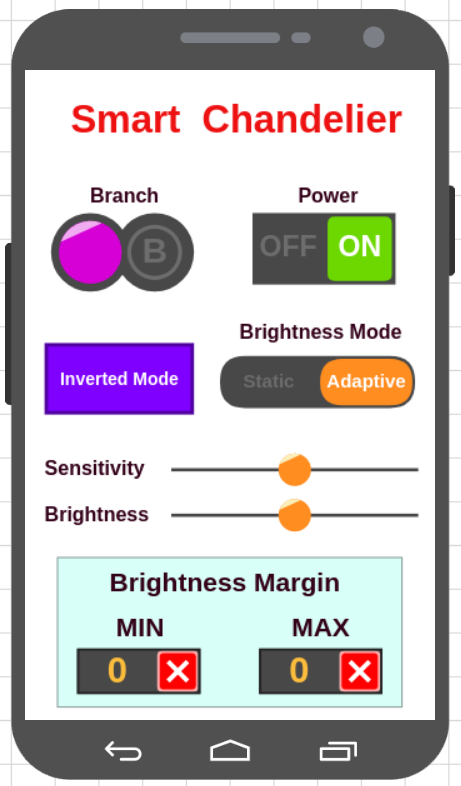
\includegraphics[scale=0.5]{figs/shcema-ma.png}
 	\caption{
 		شماتیک اپلیکیشن موبایل
 	}
 	\label{fig:schema}
 \end{figure}
 همین‌طور می‌توان کد آردویینو مربوط به این قسمت را مشاهده کرد. 

\begin{latin}
	\lstinputlisting[style={verilog-style}]{src/project.ino}
\end{latin}

\end{document}